\subsection{Problema de Kepler Newtoniano}
Si $\vec{x}_1$ y $\vec{x}_2$ son las coordenadas de $m_1$ y $m_2$ respecto a un sistema de referencia
inercial, entonces las ecuaciones de movimiento correspondientes son:
\begin{equation}
\ddot{\vec{x}}_1=-Gm_2\frac{(\vec{x}_1-\vec{x}_2)}{|\vec{x}_1-\vec{x}_2|^3} ,\label{eq:acel1}
\end{equation}
\begin{equation}
\ddot{\vec{x}}_2=-Gm_1\frac{(\vec{x}_2-\vec{x}_1)}{|\vec{x}_1-\vec{x}_2|^3} .\label{eq:acel2}
\end{equation}
Es conveniente definir una coordenada para el centro de masa $\vec{x}_{cm}$, la cual esta dada por:
\begin{equation}
\vec{x}_{\rm cm}:=\frac{m_1\vec{x}_1+m_2\vec{x}_2}{M}, \qquad M:=m_1+m_2.
\end{equation}
Con estas ecuaciones definidas se puede comprobar que a partir de \ref{eq:acel1} y \ref{eq:acel2}  el centro de masa $\vec{x}_{cm}$ es igual a cero.
\begin{equation*}
    \ddot{x}_{\rm cm} = \vec{0}.
\end{equation*}
Por lo tanto, la coordenada del centro de masa se mueve a velocidad constante. Esto permite simplificar
el problmea describiendo el movimiento desde el sistema de referencia inercial en el que el centro de masa
del sistema está en reposo y ubicado en el origen, es decir:
\begin{equation}
    \vec{x}_{\rm cm}\stackrel{!}{=}\vec{0}. \label{eq:cm}
\end{equation}
Por la condición \ref{eq:cm} implica que, en el sistema de referencia inercial del centro de masa, las coordenadas
de $m_1$ y $m_2$ están relacionadas por:
\begin{equation}
    \vec{x}_2 = -\frac{m_1}{m_2} \vec{x}_1. \label{eq:x2x1}
\end{equation}
Definiendo así una coordenada relativa dada por:
\begin{equation}
    \vec{r}:= \vec{x}_2 - \vec{x}_1 \label{eq:r}.
\end{equation}
Con esto definido, podemos escribir a la ecuación \ref{eq:x2x1} comprobar
\begin{equation}\label{eq:x12fr}
    \vec{x}_1=-\frac{m_2}{M}\vec{r}, \qquad \vec{x}_2=\frac{m_1}{M}\vec{r}.
\end{equation}
Usando estas relaciones podemos transformar las ecuaciones de movimiento \ref{eq:acel1} y \ref{eq:acel2} en ecuaciones para la coordenada relativa:
\begin{equation}
    \ddot{\vec{r}}=-GM \frac{\hat{r}}{r^2}.
    \label{eq:ddotr}
\end{equation}
Por otro lado, la energía total del sistema
\begin{equation}
    E=\frac{1}{2}m_1\vec{v}_1^2+\frac{1}{2}m_2\vec{v}_2^2-\frac{Gm_1m_2}{|\vec{x}_1-\vec{x}_2|},
\end{equation}
y el momentum angular total respecto al origen,
\begin{equation}
    \vec{L}=m_1\vec{x}_1\times\vec{v}_1+m_2\vec{x}_2\times\vec{v}_2,
\end{equation}
pueden reescribirse en términos de la coordenada relativa, resultando
\begin{equation}\label{eq:Er}
    E=\frac{1}{2}\mu \vec{v}^2-\frac{G\mu M}{r},
\end{equation}
\begin{equation}\label{eq:Lr}
    \vec{L}=\mu\,\vec{r}\times\vec{v},
\end{equation}
donde $\vec{v}:=\dot{\vec{r}}$ y $\mu:=m_1m_2/M$ es llamada la \textit{masa reducida} del sistema.\\
Los resultados de las ecuaciones \ref{eq:ddotr}, \ref{eq:Er} y \ref{eq:Lr} muestran que el movimiento relativo es equivalente
al de un cuerpo de masa $\mu$ moviendose en el potencial central fijo generado por una masa $M$ situada en el origen 
$\phi=-GM/r$. Como este potencial es central, el momentum angular total del sistema es constante a lo largo de la trayectoria. 
Como consecuencia, el movimiento está confinado al plano perpendicular $\vec{L}$. Podemos elegir el eje z normal a este plano, de modo que la trayectoria del
cuerpo satisface $\theta=\pi/2$, y entonces realizando la transformación de coordenadas rectangulares a coordenadas polares y usando $\vec{r}=r\hat{r}$ podemos
escribir la velocidad y la acelaración como:
\begin{align}
    \vec{v} & = \dot{r}\,\hat{r}+r\dot{\varphi}\,\hat{\varphi} ,\label{eq:vel1}\\
    \vec{a} & = \left(\ddot{r}-r\dot{\varphi}^2\right)\hat{r} +\left(r\ddot{\varphi}+2\dot{r}\dot{\varphi}\right)\hat{\varphi} .\label{eq:acer2}
\end{align}
Reemplazando la ecuación \ref{eq:acer2} en \ref{eq:ddotr} obtenemos
\begin{eqnarray}
    \left(\ddot{r}-r\dot{\varphi}^2\right)\hat{r}+
    \left(r\ddot{\varphi}+2\dot{r}\dot{\varphi}\right)\hat{\varphi}
    =-\frac{GM}{r^2}\hat{r}.
\end{eqnarray}
De aqui, encontramos 
\begin{eqnarray}
    \ddot{r}-r\dot{\varphi}^2&=&-\frac{GM}{r^2},\label{eq:acer3}\\
    r\ddot{\varphi}+2\dot{r}\dot{\varphi}&=&0.\label{eq:acer4}
\end{eqnarray}
Multiplicando la ecuación \ref{eq:acer4} por r, se ecuentra que el término $r^2\phi$ es constante sobre la trayectoria
\begin{eqnarray*}
    0&=&r^2\ddot{\varphi}+2r\dot{r}\dot{\varphi}\\
    &=&\frac{d\ }{dt}\left(r^2\dot{\varphi}\right),
\end{eqnarray*}
que expresa la conservación del momento angular, ya que
\begin{align*}
    \vec{L} & = \mu\,\vec{r}\times\vec{v}\\
    & = \mu\,r\,\hat{r}\times\left(\dot{r}\hat{r}+r\dot{\varphi}\hat{\varphi}
    \right)\\
    & = \mu\,r^2\dot{\varphi}\,(\hat{r}\times\hat{\varphi})\\
    & = \mu\,r^2\dot{\varphi}\,\hat{z}.
    \end{align*}
\begin{equation}
    \vec{L} == \mu\,r^2\dot{\varphi}\,\hat{z}. \label{eq:Ln}
\end{equation}
Otra cantidad conservada sobre la órbita es la energía mecánica
\begin{align}
    E&=\frac{1}{2}\mu v^2-\frac{GM\mu}{r} \label{eq:ener1}\\
    &=\frac{1}{2}\mu\dot{r}^2+\frac{1}{2}\mu r^2\dot{\varphi}^2-\frac{GM\mu}{r}.\label{eq:ener2}
\end{align}
Despejando $\dot{\varphi}$ de la ecuación \ref{eq:Ln} podemos escribir la energía mecánica sólo en términos de la variable r y constantes del movimiento:
\begin{eqnarray}
    E=\frac{1}{2}\mu\dot{r}^2+\frac{L^2}{2\mu r^2}-\frac{GM\mu}{r} .\label{eq:ener3}
\end{eqnarray}
Definiendo un potencial efectivo
\begin{equation}
    V_{\rm ef}(r):=\frac{L^2}{2\mu r^2}-\frac{GM\mu}{r},
\end{equation}
De modo que la ecuación \ref{eq:ener3} pueda ser escrita como la ecuación de conservación de la energía de un movimiento unidimensional:
\begin{equation}
    E=\frac{1}{2}\mu\dot{r}^2+V_{\rm ef}(r) . \label{eq:EVef}
\end{equation}
    El potencial efectivo $V_{\rm ef}(r)$ posee un cero en
\begin{eqnarray}
    r_{\rm c}=\frac{L^2}{2GM\mu^2} ,\label{eq:cero1}
\end{eqnarray}
y además posee un mínimo en
\begin{eqnarray}
r_{\rm min}=\frac{L^2}{GM\mu^2}=2r_{\rm c},\label{eq:rmin}
\end{eqnarray}
tal que
\begin{eqnarray*}
V_{\rm ef, min}=-\frac{G^2M^2\mu^3}{2L^2}<0.
\end{eqnarray*}
Además, el comportamiento asintótico del potencial efectivo es
\begin{eqnarray*}
\lim_{r\to\infty}V_{\rm ef}(r)&\approx&-\frac{GMm}{r}\rightarrow 0,\\
\lim_{r\to 0}V_{\rm ef}(r)&\approx&\frac{L^2}{2mr^2}\rightarrow +\infty .
\end{eqnarray*}
\begin{figure}[H]
    \centering
    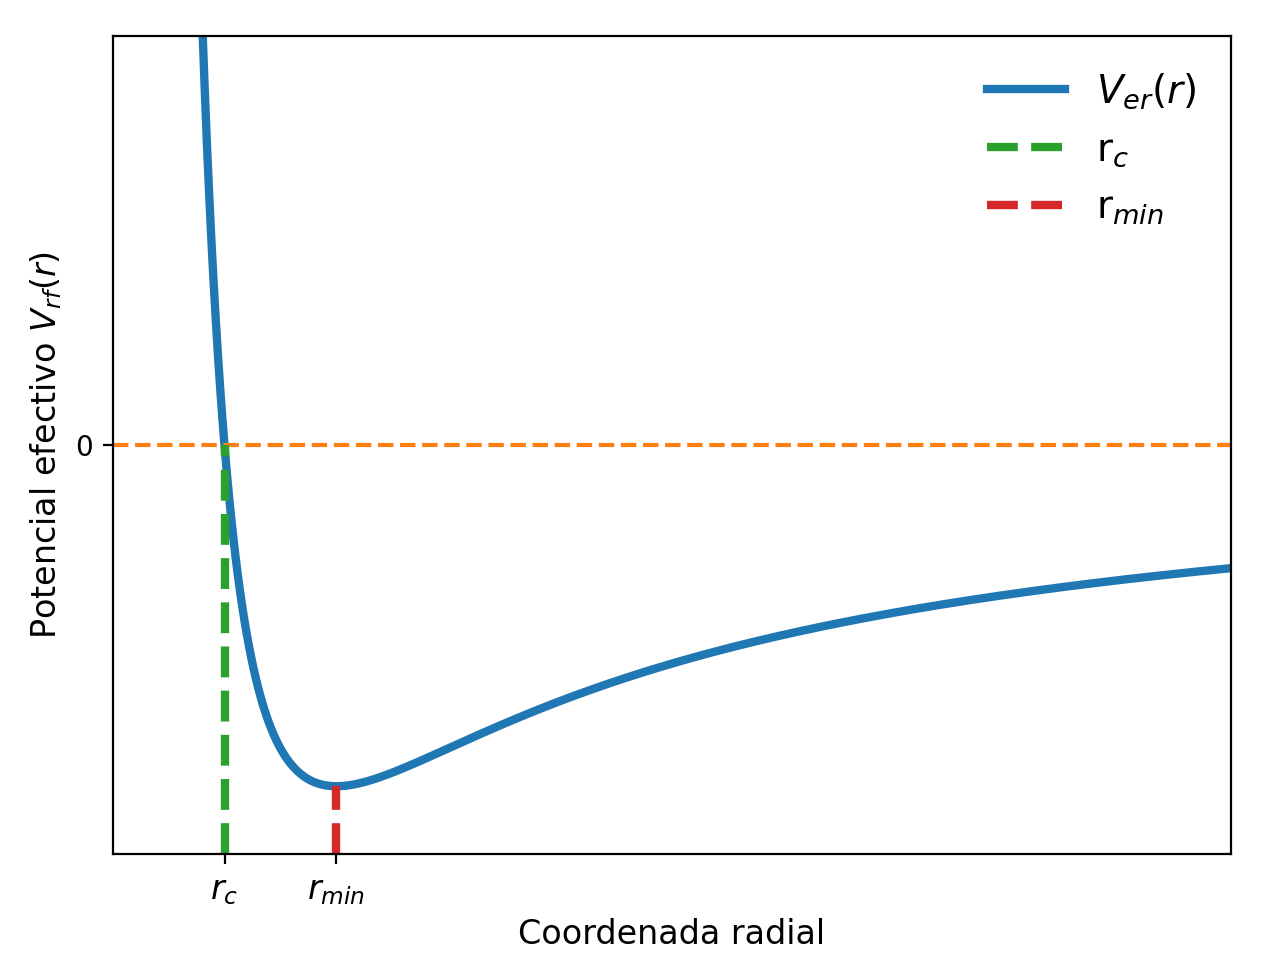
\includegraphics[scale=0.6]{images/Pot_efe.png}
    \caption{Potencial newtoniano efectivo, las constantes $L,G,M,\mu$ igualadas a 1}
\end{figure}
Así para un valor de $L$ dado, tenemos que:
\begin{enumerate}
    \item Si $E_1>0$, una part'icula proveniente del infinito alcanza un radio
    mínimo $r_1$, donde $\dot{r}^2=0$, y luego vuelve a infinito.
    \item Si $V_{\rm ef, min}<E_2<0$ la trayectoria es ligada, variando la distancia entre dos puntos de retorno $r_2$ y $r_3$, de modo que $r_2<r<r_{3}$.
    \item Si $E_{3}=V_{\rm ef, min}$ la partícula
    describe un movimiento circular de radio dado por la ecuación \ref{eq:rmin}. Este caso
    corresponde al mínimo del potencial, por lo que es un
    movimiento estable.
    \item Finalmente, no existen trayectorias con $E<V_{\rm ef, min}$ ya que la ecuación \ref{eq:EVef} requiere que $E\ge V_{\rm ef}$.
\end{enumerate}
Determinando la forma de la trayectoria, descrita por la dependencia de la coordenada radial $r$ en términos de la coordenada angular $\varphi$. Asumiendo $r=r(\varphi)$ podemos escribir
\begin{eqnarray}
    \dot{r}=\frac{dr}{d\varphi}\dot{\varphi}=\frac{L}{\mu r^2}\frac{dr}{d\varphi}.
    \label{eq:dotr}
\end{eqnarray}
Reemplazando en la ecuación \ref{eq:ener3} la ecuación \ref{eq:dotr} obtenemos
\begin{equation}
    \frac{1}{r^4}\left(\frac{dr}{d\varphi}\right)^2=\frac{2\mu E}{L^2}+\frac{2GM\mu^2}{L^2r}-\frac{1}{r^2}.\label{eq:ener4}
\end{equation}
Con un cambio de variable $u:=1/r$, entonces la ecuación \ref{eq:ener4}
\begin{equation}
    (u')^2=\frac{2\mu E}{L^2}+\frac{2GM\mu^2}{L^2}\,u-u^{2
    },\label{eq:ener5}
    \end{equation}
derivandi la ecuación \ref{eq:ener5} se encuentra la ecuación de movimiento para $u$ en funcion de $\varphi$
\begin{equation}
    u''+u=\frac{GM\mu^2}{L^2}.\label{eq:EC1}
\end{equation}
La integración de la ecuación \ref{eq:EC1} es directa ya que corresponde a un oscilador armónico con un término forzante constante
\begin{equation}
    u(\varphi)=\frac{GM\mu^2}{L^2}\left(1+e\cos
    (\varphi-\varphi_0)\right)\label{eq:CON1}
\end{equation}
donde reemplazando la solución \ref{eq:CON1} en \ref{eq:ener5}
\begin{equation}
    e=\sqrt{1+\frac{2L^2E}{G^2M^2\mu^3}}, \label{eq:ex}
\end{equation}
es la excentricidad dela orbita y $\phi_0$ es una constante de integración correspondiente a la orientación inicial relativa al eje x.
Si $-G^2M^2\mu^2/2L^2<E<0$ entonces $0<e<1$, y la cónica es una elipse.\\
El semieje mayor de la órbita es 
El semieje mayor de la 'orbita,
\begin{equation*}
a=\frac{1}{2}\left(r_{\rm max}+r_{\rm min}\right),
\end{equation*}
puede ser escrito en términos de las constantes de movimiento a partir de las ecuaciones \ref{eq:CON1} y \ref{eq:ex}
\begin{align*}
    a & = \frac{1}{2}\left(\frac{1}{u_{\rm min}}+\frac{1}{u_{\rm max}}\right) \\
    & = \frac{1}{2}\left(\frac{L^2}{GM\mu^2}\frac{1}{(1+e)}+\frac{L^2}{GM\mu^2}\frac{1}{(1-e)}\right) \\
    & = \frac{L^2}{GM\mu^2}\frac{1}{(1-e^2)} \\
    & = -\frac{GM\mu}{2E}.
    \end{align*}
\begin{equation}
    a= -\frac{GM\mu}{2E}. \label{eq:aE}
\end{equation}
Con esto, podemos escribir la solución de la ecuación \ref{eq:CON1} como 
\begin{equation}
    u(\varphi)=\frac{1}{a(1-e^2)}\left[1+e\cos
    (\varphi-\varphi_0)\right],
    \end{equation}
    o, en términos de la coordenada radial relativa,
    \begin{equation}\label{eq:rphi}
    r(\varphi)=\frac{a(1-e^2)}{1+e\cos(\varphi-\varphi_0)}.
\end{equation}
La evolución temporal de la órbita puede ser determinada implícitamente de la forma siguiente. Definamos la variable auxiliar
$s$ por
\begin{equation}\label{eq:rs}
    r=:a(1-e\cos s).
\end{equation}
A partir de esto podemos usar la ecuación \ref{eq:rphi} para encontrar una relación entre $\varphi$ y $s$ sobre la órbita.
De esta forma, obtenemos 
\begin{equation}\label{eq:phiscos}
    \cos(\varphi-\varphi_0)=\frac{\cos s -e}{1-e\cos s},
\end{equation}
y a partir de aqui
\begin{equation}\label{eq:phissen}
    \sen(\varphi-\varphi_0)=\sqrt{1-e^2}\,\frac{\sen s}{1-e\cos s}.
\end{equation}
Derivando la ecuación \ref{eq:phiscos} respecto a $s$ y usando la ecuación \ref{eq:phissen} obtenemos 
\begin{equation*}
    \frac{d\varphi}{ds}=\frac{\sqrt{1-e^2}}{1-e\cos s}.
\end{equation*}
Con esto, podemos expresar el momento angular de la ecuación \ref{eq:Ln} en términos de $s$;
\begin{align*}
    L & = \mu r^2 \frac{d\varphi}{dt} \\
    & = \mu r^2 \frac{d\varphi}{ds}\frac{ds}{dt} \\
    & = \mu a^2\left(1-e\cos s\right)^2 \frac{d\varphi}{ds}\frac{ds}{dt} \\
    & = \mu a^2\sqrt{1-e^2}\left(1-e\cos s\right) \frac{ds}{dt} .
\end{align*}
Por lo tanto:
\begin{align*}
    1-e\cos s & = \frac{L}{\mu a^2\sqrt{1-e^2}} \frac{dt}{ds} \\
    & =: \omega_0 \frac{dt}{ds},
\end{align*}
\begin{equation}
    1-e\cos s =: \omega_0 \frac{dt}{ds}, \label{eq:dtds}
\end{equation}
donde hemos introducido el término $\omega_0$, con unidades de frecuencia, que usando la ecuación \ref{eq:ex} satisface 
\begin{equation}\label{Kepler3}
    \omega_0^2=\frac{GM}{a^3}.    
\end{equation}
La relación de la ecuación \ref{eq:dtds} puede integrarse directamente respecto a $s$. Eligiendo la condición inicial $s=0$ para $t=0$ obtenemos
\begin{equation}\label{eq:ts}
    \omega_0(t-t_0)=s-e\sen s.
\end{equation}
Las expresiones de las ecuaciones \ref{eq:ts}, \ref{eq:rs}, \ref{eq:phiscos} y \ref{eq:phissen} suministra una \textit{solución paramétrica} para la órbita.
A partir de la ecuación \ref{eq:rphi} vemos que $r(\varphi)$ es periodica con periodo $\Delta\varphi=2\pi$. Además, de las ecuaciones \ref{eq:rs} y \ref{eqphiscos} 
vemos que este periodo corresponde a un cambio en $2\pi$ en la variable auxiliar $s$. 
Finalmente, la relación \ref{eq:rs} implica que esta periodicidad corresponde a un intervalo de tiempo
\begin{equation}
T=\frac{2\pi}{\omega_0},
\end{equation}
que es entonces el \textit{periodo orbital}. Con esto la ecuación \ref{eq:Kepler3} implica la \textit{tercera ley de Kepler}.